\documentclass[addpoints]{exam}

\usepackage{caption}
\usepackage{graphbox}
\usepackage{hyperref}
\usepackage{listings}
\usepackage{multirow}
\usepackage{ragged2e}
\usepackage{subcaption}
\usepackage{tabularx}
\usepackage{xcolor}

% Header and footer.
\pagestyle{headandfoot}
\runningheadrule
\runningfootrule
\runningheader{CS 201 Data Structures II}{HW 3: Graphs}{Spring 2020}
\runningfooter{}{Page \thepage\ of \numpages}{}
\firstpageheader{}{}{}

% \qformat{{\large\bf \thequestion. \thequestiontitle}\hfill[\totalpoints\ points]}
\qformat{{\large\bf \thequestion. \thequestiontitle}\hfill}
\boxedpoints

\printanswers

\graphicspath{{images/}}

\newcommand\colheader[1]{\multicolumn{1}{c}{#1}} % Note: no vertical bars

% Colored Python listing from https://www.overleaf.com/learn/latex/Code_listing
\definecolor{codegreen}{rgb}{0,0.6,0}
\definecolor{codegray}{rgb}{0.5,0.5,0.5}
\definecolor{codepurple}{rgb}{0.58,0,0.82}
\definecolor{backcolour}{rgb}{0.95,0.95,0.92}
 
\lstdefinestyle{mystyle}{
    backgroundcolor=\color{backcolour},   
    commentstyle=\color{codegreen},
    keywordstyle=\color{magenta},
    numberstyle=\tiny\color{codegray},
    stringstyle=\color{codepurple},
    basicstyle=\ttfamily\footnotesize,
    breakatwhitespace=false,         
    breaklines=true,                 
    captionpos=b,                    
    keepspaces=true,                 
    numbers=left,                    
    numbersep=5pt,                  
    showspaces=false,                
    showstringspaces=false,
    showtabs=false,                  
    tabsize=2
}
\lstset{style=mystyle}

\title{Homework 3: Graphs}
\author{CS 201 Data Structures II\\Habib University\\Spring 2020}
\date{Due: 1830h on Friday, 5 March}

\begin{document}
\maketitle

\begin{figure}[h]
  \centering
  \begin{subfigure}{.48\textwidth}
    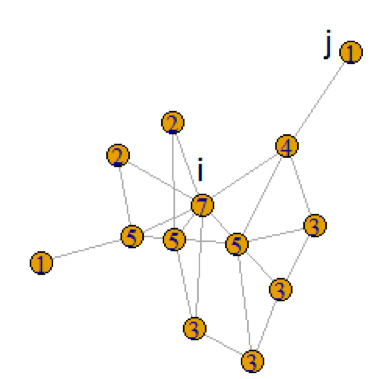
\includegraphics{fig1}
    \caption{$i$ is the most popular vertex in the network with a degree of 7.}
    \label{fig1}
  \end{subfigure}
  \begin{subfigure}{.48\textwidth}
    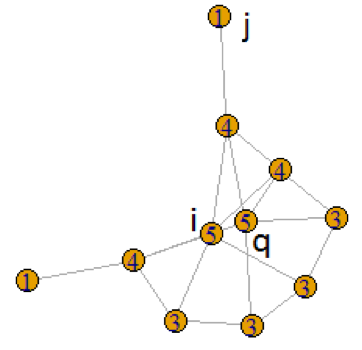
\includegraphics{fig2}
    \caption{This network has 2 most popular vertices, $i$ and $q$, each having a degree of 5.}
    \label{fig2}
  \end{subfigure}
  % \begin{subfigure}{.3\textwidth}
  %   \includegraphics[width=\textwidth]{pool-only-blue}
  %   \caption{The original image with only the blue channel turned on.}
  % \end{subfigure}
  \caption{Two networks are shown with the nodes in each labeled with its degree.}
  \label{fig:figs}
\end{figure}

The world we live in is an inter-connected system and many aspects of it can be represented by a graph, or a \textit{network}. A good example is the World Wide Web (WWW) which is an inter-connected system of web-pages in which each vertex represents a page and an edge represents a direct link between two web pages.

\textit{Network Science} is the study of the networks that appear in different domains, e.g. in social, technological, and biological disciplines. It finds application in many fields including sociology, physics, mathematics, biology, economics, and computer science. The aim is to identify underlying common principles in the formation of networks and explore why they vary in some cases. This is done through exploration of networks to study structural patterns and to identify variations.

The field has undergone tremendous growth especially after ground-breaking discoveries of \textit{small-world} and \textit{scale-free} properties in network models. Traditional graph theoretic properties take on added significance in network science. For example, the degree of a vertex can be interpreted as the \textit{popularity} of the vertex--in a social network, a person with a higher value of the degree is a person with a lot of friends.  Similarly, \textit{clustering coefficient} is used to quantify how closely vertices are connected to each other within a neighborhood. The \textit{degree distribution} of a graph describes the structure of the graph, i.e. whether it has a few prominent vertices or \textit{hubs}.

In this assignment, we are going to explore (and implement) some of the measures used in network science and apply them to a few popular datasets.

\section{Measures}

We look at 5 measures: \textit{degree centrality}, \textit{clustering coefficient}, \textit{average neighbor degree}, \textit{Jaccard similarity}, and \textit{popular distance}.

\paragraph{Degree Centrality}
\textit{Centrality} provides a measure of the \textit{importance} of a vertex or edge. \textit{Degree centrality} uses the degree of a vertex, i.e. the number of connections of the vertex, as the measure. To compare across networks of different sizes, i.e. with different number of vertices, the degree is normalized by the total number of vertices in the network.
\[
  C_D(i) = \frac{k_i}{n-1}
\]
where $i$ is the subject vertex, $k_i$ is its degree, and $n$ is the total number of vertices in the network.

\paragraph{Clustering Coefficient}
\textit{Clustering coefficient} is used to quantify the connectivity of vertices in a graph. The \textit{local} clustering coefficient for an individual vertex, $i$, can be used to determine whether a graph is a \textit{small-world network} and is calculated as
\[
  C_i=  \frac{L_i}{\frac{k_i (k_i-1)}{2}}
\]
where $k_i$ is the number of neighbors of $i$ and $L_i$ is the total number of edges between the $k_i$ neighbors of $i$. The denominator indicates the maximum possible edges among the $k_i$ neighbors. If all the neighbors are connected with each other, $C_i$ will be 1, and if there are no common friends among the neighbors, $C_i$ will be 0. The average clustering coefficient of a network with $n$ vertices is the average of all the local clustering coefficients.
\[
  \overline{C}=  \frac{1}{n} \sum_i C_i
\]

\paragraph{Average Neighbor Degree}

The degree of a vertex describes how famous or popular it is in the network. \textit{Average neighbor degree} tells whether the vertex is surrounded by famous vertices. For a vertex, $i$, it is calculated as
\[
  K_i = \frac{1}{|N(i)|} \sum_{j\in N(i)} k_j
\]
where $N(i)$ is the set of neighbours of $i$ and $k_j$ is the degree of node $j$.

\paragraph{Jaccard Similarity}

\textit{Jaccard Similarity} is used to determine the similarity of two vertices to each other. Vertices $i$ and $j$ are more similar if they have more common friends. Jaccard similarity between 2 vertices, $i$ and $j$, is calculated as:
\[
  J(i,j) =  \frac{|N(i) \cap N(j)|}{|N(i) \cup N(j)|} = \frac{|N(i) \cap N(j)|}{|N(i)|  + |N(j)| - |N(i) \cap N(j)|}
\]
where $N(i)$ and $N(j)$ are the sets of neighbors of $i$ and $j$ respectively.

\paragraph{Popular Distance}
Another measure to find the importance of a vertex in a network is its distance from the most popular vertex of the network. The \textit{popular distance} of a vertex $i$ is the length of the shortest path from $i$ to the vertex with the maximum degree. If the network contains more than one vertex with maximum degree then the minimum shortest path is considered. For example, the popular distance of vertex $j$ in Figure \ref{fig1} is 2 as that is the length of the shortest path from $j$ to $i$. In Figure \ref{fig2}, the popular distance of $j$ is again 2 as it is at a distance of 2 from each of $i$ and $q$ which are the 2 most popular vertices in the network.

\section{Datasets}

For this homework, we use three different datasets: ``Zachary's Karate Club'', ``Coauthorships in Network Science'', and ``High Energy Physics - Theory collaboration network''. For the figures below, zoom into the figure with your PDF viewer to see more detail.

\noindent\begin{tabular}{*{2}{p{.48\textwidth}}}
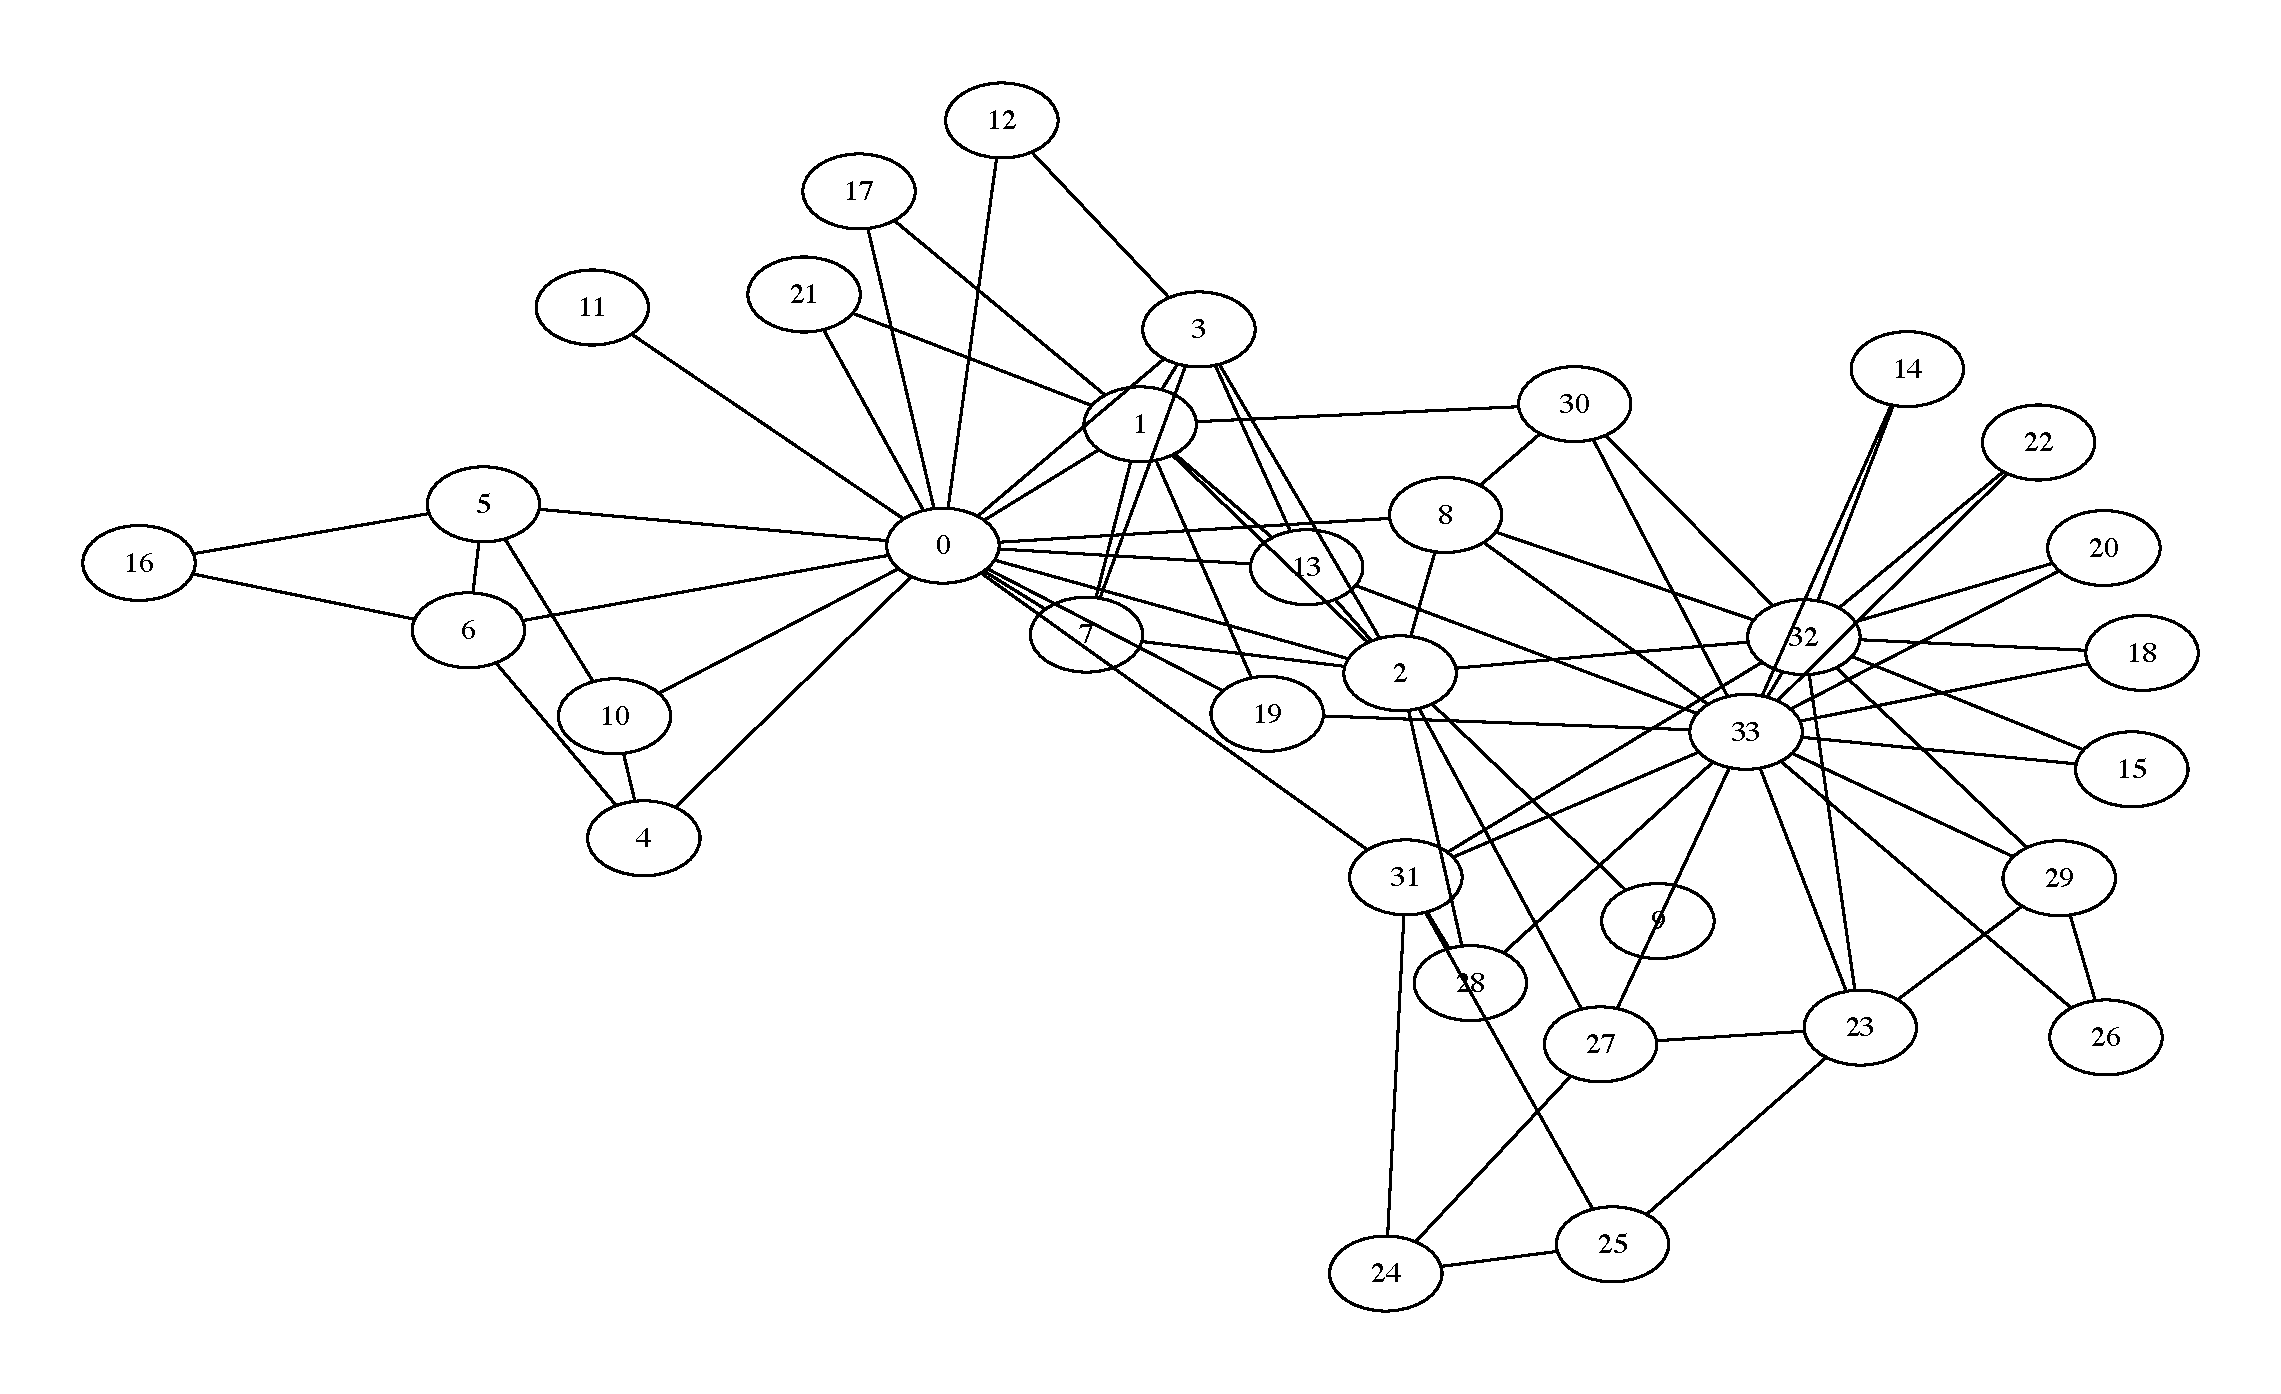
\includegraphics[width=.5\textwidth,align=t]{karate} & 
\paragraph{Zachary's Karate Club} is probably the most presented network at network science conferences! The network represents social ties among the members of a karate club at a university. Each vertex represents a member of the club and an edge between two vertices indicates that the corresponding members are friends. The network is undirected and unweighted.
\end{tabular}

\paragraph{Coauthorships in Network Science} is a collaboration network of coauthorships between scientists in the area of network theory and experiments.  Each vertex represents an author and an edge between vertex $i$ and vertex $j$ indicates that the corresponding authors have co-authored a paper. The network is undirected and unweighted. See Figure \ref{fig:netsci} for a visualization.

\paragraph{High Energy Physics - Theory collaboration network} is a collaboration network of coauthorships between scientists in the area of High Energy Physics – Physics. The network is constructed from the e-print arXiv for the papers submitted to High Energy Physics - Theory category. The network is undirected and weighted where the weight of an edge represents the number of papers co-authored by both authors involved in the edge. Edge weights are normalized. See Figure \ref{fig:hep} for a visualization.

\begin{figure}
  \centering
  \includegraphics[width=\textwidth]{netsci}
  \caption{Coauthorships in Network Science}
  \label{fig:netsci}
\end{figure}

\begin{figure}
  \centering
  \includegraphics[width=\textwidth]{hep}
  \caption{High Energy Physics - Theory collaboration network}
  \label{fig:hep}
\end{figure}
\section{Tasks}

Your task is to go over the provided files and fill in the required functionality.
\begin{description}
\item[\texttt{networks.py}] contains network operations that operate on a \texttt{Graph}. All methods currently contain \texttt{pass} which will have to be replaced by you. The exception is \texttt{visualize} which is implemented. When this function executes successfully, the visualization is automatically stored in the files \texttt{Graph}.gv and \texttt{Graph.gv.pdf}. Do not add these to your repository.
\item[\texttt{graphs.py}] contains a complete implementation of \texttt{Edge} which represents an undirected edge and the interface of \texttt{Graph}. You have to implement the \texttt{Graph} interface using 3 different classes \texttt{SetGraph}, \texttt{AdjacencyMatrix}, and \texttt{AdjacencyList} that store a graph respectively as 2 sets, an adjacency matrix, and an adjacency list. Do not alter the code already provided.
\end{description}

Also go over the files in the \texttt{datasets} folder. Each file represents a network as en \texttt{edge list}. Each line contains the 2 endpoints of an edge. Each vertex is represented by an integer. For some networks, each line also contains a weight as a floating point number. Note that the vertex numbers need not begin at 0 and need not be contiguous. A Graph is instantiated with a \texttt{str} instance representing the content of such a file.

You may use the given networks to test your code. 

\section*{Credits}

This homework and related files are courtesy of \href{http://qasimpasta.info}{Muhammad Qasim Pasta}.

\end{document}

%%% Local Variables:
%%% mode: latex
%%% TeX-master: t
%%% End:
